\renewcommand{\thetable}{\arabic{chapter}.\arabic{table}}
\renewcommand{\thefigure}{\arabic{chapter}.\arabic{figure}}
\chapter[Pendahuluan]{\uppercase{Pendahuluan}}
\setcounter{chapter}{1}
\renewcommand{\thesection}{\norsize\bfseries {\arabic{chapter}.\arabic{section}}}
\titleformat{\section}
{\norsize\bfseries}{\thesection}{1em}{}

\section{Latar Belakang Masalah}\index{Latar Belakang Masalah}
\begin{sloppypar}
    Ini adalah contoh membuat sebuah paragraf yang merujuk pada Gambar \ref{fig:1.1}. Perhatikan cara membuat gambar dan cara merujuknya. Selain itu dicontohkan bagaimana membuat tulisan cetak miring atau \emph{italyc} jika tulisan berbahasa asing, juga cetak \textbf{tebal} maupun \underline{bergaris bawah}. Untuk sitasi gunakan perintah \\citep\{identifier\} nanti hasilnya seperti ini \citep{Abadi.2016}. Untuk menggunakan subscipt dan seprtscrip contohnya $NO_3^-$.  Sedangkan contoh tabel bisa dilihat patda Tabel \ref{tbl:1.1}.
\end{sloppypar}

\begin{table}
    \caption{\label{tbl:1.1}Contoh sebuah tabel}
    \footnotesize\rm
    \begin{tabular*}{\textwidth}{@{}l*{12}{@{\extracolsep{0pt plus12pt}}l}}
    \hline
    Karakter & Indikator\\
    \hline
    Perhatian (\emph{mindfullness}) & bijaksana, kesadaran diri, pengendalian diri, aktualisasi diri,  observasi, \\ & refleksi, kesadaran, kasih sayang, bersyukur, empati, peduli, tumbuh, \\ & berwawasan, memiliki pandangan \\
    Rasa Ingin Tahu  (\emph{coriosity})& berpikiran terbuka, mengeksplorasi, bergairah,  pengarahan diri, \\ & motivasi, inisiatif, inovative, antusias, mempertanyakan, mengapresiasi \\
    Keberanian (\emph{courage}) & berani, menentukan, ketabahan, percaya diri, berani mengambil resiko, \\ &gigih, kuat, optimis, menginspirasi, energik, bersemangat, gembira,  \\
    \hline
    \end{tabular*}
\end{table}

\begin{figure}[h]
    \centerline{\hbox{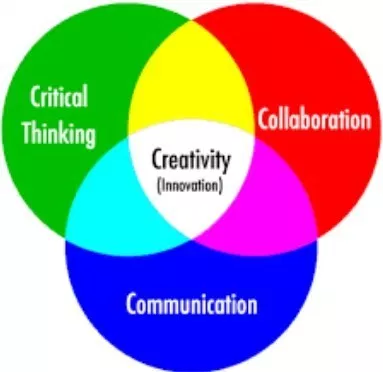
\includegraphics[scale=0.5]{bab1/4C.png}}}
    \caption{\label{fig:1.1}Contoh Gambar}
\end{figure}

\section{Tujuan}


\section{Manfaat}


